\documentclass[a4paper,11pt]{kth-mag}
\usepackage[T1]{fontenc}
\usepackage{textcomp}
\usepackage{lmodern}
\usepackage{graphicx}
\usepackage[utf8]{inputenc}
\usepackage[swedish,english]{babel}
\usepackage{modifications}
\usepackage{algorithmicx}

\usepackage{amsmath}
\usepackage{amssymb}
\usepackage{algpseudocode}

\usepackage{hyperref}

% http://library.uwl.ac.uk/find/guides/general/harvard_reference.html

\title{Evolution of Artificial Brains in Simulating Animal Behaviour}
\subtitle{Comparing radial basis, linear and random functions for decision-making}
\foreigntitle{Evolution av artificiella hjärnor vid simulering av djurs beteende}
\author{Björn Tegelund\\Johan Wikström}
\date{November 2003}
\blurb{Bachelor's Thesis at CSC\\Supervisor: Petter Ögren\\Examiner: Mårten Björkman}
\trita{TRITA xxx yyyy-nn}
\begin{document}
\frontmatter
\pagestyle{empty}
\removepagenumbers
\maketitle
\selectlanguage{english}
\begin{abstract}
  This is a skeleton for KTH theses. More documentation
  regarding the KTH thesis class file can be found in
  the package documentation.

\end{abstract}
\clearpage
\begin{foreignabstract}{swedish}
  Denna fil qer ett avhandlingsskelett.
  Mer information om \LaTeX-mallen finns i
  dokumentationen till paketet.

\end{foreignabstract}
\clearpage
\tableofcontents*
\mainmatter
\pagestyle{newchap}
\chapter{Introduction}

\section{Background}

Genetic algorithms are algorithms that emulate evolution in order to achieve a optimal solution to a problem. 
These algorithms have many uses and it is therefore interesting to investigate whether the phenomena which occur in nature due to evolution also occur when using genetic algorithms. In nature evolution has spawned a wide variety
of survival strategies such as adaptation, camouflaging colours and mimicry. Genetic algorithms, however, are 
 simplified mathematical models of these mechanisms which means that these phenomena might not occur 
at all.

\section{Scope and Objectives}

The main objective is to compare brains for simulating animal behaviour using radial-basis functions and linear functions. As a baseline a brain which makes random decisions will also be used. To train the animals genetic algorithms will be used. The genetic algorithms provide the genes which will then be used in their brains to make decisions. Statistics such as learning speed, choice of strategy and how well the creatures are able to adapt to their surroundings will then be analysed. 

The animals will be given different tasks to do in each experiment, ranging from simply gathering food to avoiding predators to mimicking things in the world to survive. In each experiment the three brain architectures are compared and contrasted. By doing these simulations the goal is to find out the pros and cons of both brains using radial-basis functions and linear functions, when used for simulating artificial intelligence in this way.

It is also of interest to look closer at how complex of a task a brain using linear functions is able to solve, and in the cases where it is not able to solve the problem completely, compare its performance to the random brain.

% TODO: What did we manage to simulate?
%  Forcing them to adapt certain genetic phenomena such as adaptation (learning), co-evolution and extinction, mimicry, group forming and co-operation prioritised in the order presented (as increasingly complex behaviour and difficulty to simulate).

\section{Achievements}

\chapter{Technical Overview}

\section{Genetic Algorithms}

\subsection{Overview}
What are genetic algorithms?\\
How are they typically used?\\
How do they relate to genetics and evolution?\\
Overview of algorithm\\

Genetic algorithms are a way of approximating solutions to NP-hard problems, a group of problems that are extremely computationally expensive. They are a form of machine learning algorithms typically used to solve problems with a large or complex search space and where other machine learning algorithms fail \cite{marsland}. Genetic algorithms mimic natural selection in nature by defining a set of genomes, or individuals, where each genome represents a possible solution to the given problem. This genome is commonly stored as a string of 0:s and 1:s or as a list of floating point values. This set of genomes undergoes several iterations, or generations, of small improvements by fitness evaluation, selection, mutation and crossover. These operators all have equivalents in natural evolution and eventually the genomes will converge to a solution which represents a local minima in the search space. The advantage of genetic algorithms is that the crossover operator enables a wider search over the problem domain than many other approaches, using less calculations \cite{holland}. In the following subsections, the most crucial parts of the genetic algorithm will be explained and in figure \ref{algorithm-overview}   an overview of the genetic algorithm in pseudo code is depicted.

\begin{figure}
\begin{algorithmic}
\State $ S \gets $ a random distribution of genes
    \While {the genes have not converged towards a solution}

        \State $F\gets fitness(S)$
		\Comment Calculate fitness values for all $s \in S$
		\State $X \gets select(S,F)$
		\Comment Get a multiset of S using fitness values
		\State $C \gets crossover(X)$
		\Comment Apply crossover operator on multiset
		\State $M \gets mutate(C)$
		\Comment Apply mutation operator on crossed genes
		\State $S \gets M$
		\Comment Restart with the new generation
    \EndWhile
\end{algorithmic}
\caption{An overview of the genetic algorithm used in the experiments}
\label{algorithm-overview}
\end{figure}

\subsection{Fitness}
Fitness is the only means of measuring the success of the solution. In nature, fitness is simply determined by the number of offspring produced by the individual and the percentage of that offspring which survives long enough to generate new offspring. In genetic algorithms however, the fitness function can be any value that describes each individual's success at solving the problem at hand and genetic algorithms can get significant performance advantages by simply selecting the correct fitness function \cite{marsland}. The fitness function should be strictly positive for all inputs and preserve some form of relative internal ordering of the individuals. In most problems there are multiple choices of fitness functions and the best choice of fitness function is unique for every problem. For this reason, a lot of different fitness functions were tried before settling for simply the life length of the individuals. Another reason for choosing this fitness function is that it is general, which allows the creatures to freely choose strategies.

\subsection{Selection}
Selection is the process of selecting which organisms that should be allowed to reproduce and in what proportions. In nature, selection is closely tied to fitness, the fittest individual is also "selected" most often, but in genetic algorithms there are several different ways to model this selection process. A good fitness function should strike a balance between favouring the fittest individuals and allowing less fit individuals to survive in a reduced number.  One trivial selection function could be to simply select all individuals that pass a certain fitness threshold \cite{marsland} [TROR DET STOD DÄR IAF]. This is a bad idea, however, since there are few ways to determine the correct threshold value. In the beginning of the evolution, a high threshold will exclude most of the genes due to low general fitness and this will lead to a fast reduction of genetic variation. In the later stages of the evolution all individuals will pass the threshold, rendering the selection function useless.

A better approach is the so called roulette wheel selection where each individual is mapped to an area of a "roulette wheel". A larger fitness value means a larger area on the roulette wheel and the selection function simply generates random values corresponding to the areas of this roulette wheel. In this way, the individuals are chosen based on a biased stochastic variable and there is room for individuals with high fitness to dominate as well as for individuals with low fitness to be included by chance. Figure \ref{roulettewheelpic} shows what this can look like, and how its similarities to a traditional roulette wheel.

\begin{figure}
\centering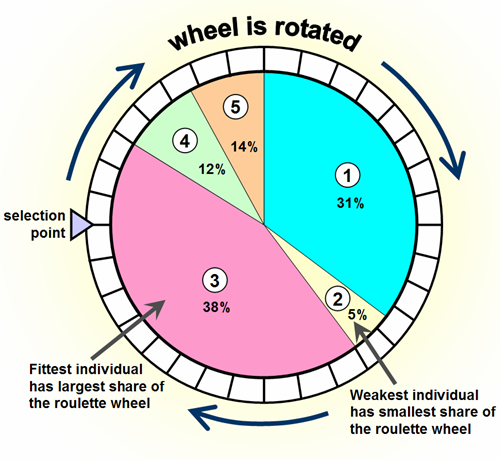
\includegraphics[scale=0.9]{roulettewheel.png}
\caption{A visual representation of how the roulette wheel selection algorithm works.}
% Beh�ver vi source till detta? Hittades h�r: http://www.edc.ncl.ac.uk/highlight/rhjanuary2007g02.php/
\label{roulettewheelpic}
\end{figure}

Undrar om vi ska skriva något om NSGA II...
 
\subsection{Mutation}
Mutation is a random, usually small, change of an individuals genome. In nature this typically occurs spontaneously when new cells are formed. In genetic algorithms it is usually implemented as a small probability for each gene to mutate. When the genome consists of a series of 0:s and 1:s, the mutation operator is simply a flip of that bit and when the genes consist of floating point values, the mutation can be an addition or multiplication of a random value. If the mutation rate is too high, it becomes very hard to reach convergence since the good solutions are mutated into averaged solutions.

\begin{figure}
\centering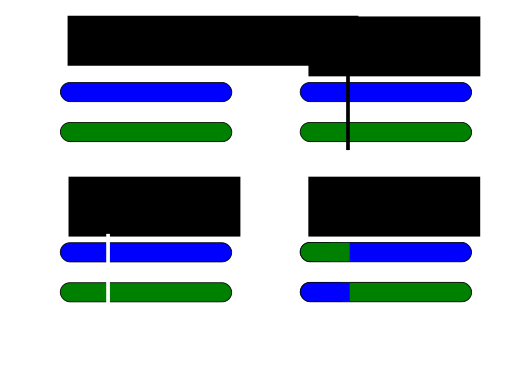
\includegraphics[scale=0.5]{crossover}
\caption{A schematic drawing showing single point crossover of two genomes.}
\label{crossover-figure}
\end{figure}

\subsection{Crossover}
Crossover is the operation of combining two genomes into two new genomes. One common crossover operator is known as  single point crossover and it consists of splitting two genomes at the same position and merging the split parts into two new genomes. The split position is chosen randomly and the two new genomes share no genes with each other. This process is displayed in Figure \ref{crossover-figure} There is also the possibility of using multiple point crossover where there are multiple splitting positions as well as uniform crossover where each gene can be exchanged with a certain probability.

\section{Radial Basis Functions}
\subsection{Overview}

\begin{figure}
\centering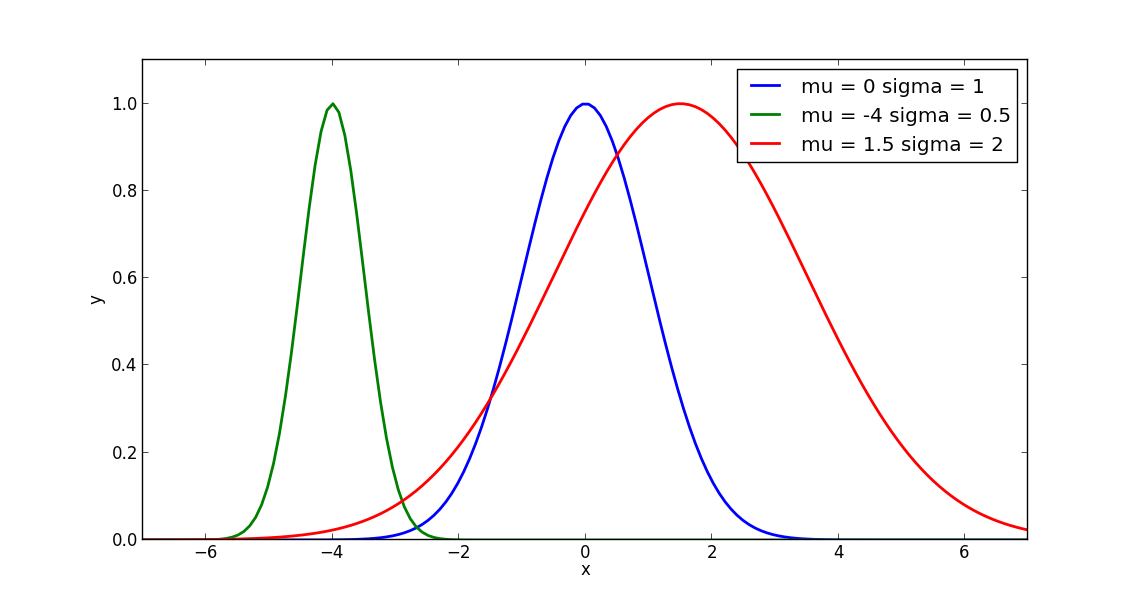
\includegraphics[scale=0.5]{rbf_1d.png}
\caption{Three one-dimensional RBFs with varying $\mu$ and $\sigma$ values.}
\label{3-rbf-functions}
\end{figure}

A radial basis function (RBF) is a bell-shaped function whose value depends on the distance from some origin, denoted $\mu$ in the formula.  Radial basis functions are commonly used in neural networks as a way to encode input information. They are favourable to use as they have locality, something which linear functions do not. In particular they are used for function approximation, as any function can be approximated as the sum of a number of weighted radial basis functions. A property of radial basis functions which can both be interpreted as an advantage and disadvantage is that their value never exceeds a given constant, compared to a linear function which can grow to infinitely high or low numbers.

Radial basis functions are commonly implemented using a formula such as \ref{RBF_1}, which is a three-dimensional function centred around $(\mu _{x}$, $\mu _{y}$, $\mu _{z})$. The width of the bell-curve in each dimension is determined by $\sigma _{x}$, $\sigma _{y}$ and $\sigma _{z}$ respectively.

\begin{figure}
\begin{equation}
f(x,y,z) = \exp(-(\frac{(x-\mu_{x})^{2}}{2 \sigma _{x}^{2}})) + \exp(-(\frac{(y-\mu_{y})^{2}}{2 \sigma _{y}^{2}})) + \exp(-(\frac{(z-\mu_{z})^{2}}{2 \sigma _{z}^{2}}))
\end{equation}
\caption{A sum of three radial basis functions, corresponding to three input values.\label{RBF_1}}
\end{figure}

\chapter{Implementation}
\section{Model}
\subsection{Simulation in Python}

Python was chosen as the language to implement our simulation in as it is a high-level language suited for quickly building prototypes. It also has an abundance of third-party libraries which helps reduce implementation time significantly. A third-party library called DEAP (Distributed Evolutionary Algorithms in Python) was used for the evolutionary algorithms. DEAP proved to be flexible enough for the task as it allows the user to define their own selection, mutation and crossover algorithms as well as mixing them with the accompanying built-in algorithms. Pygame and Matplotlib were used for graphical rendering, Pygame for rendering the actual simulation and Matplotlib for producing graphs from the extracted data. To increase performance Pypy, Numpy and Python's built-in support for multiprocessing were used to decrease runtime significantly. For a comprehensive list of the tools used, please see Appendix \ref{list-of-third-party-tools}.

Square world with walls, circular inhabitants with antennae\\
Good and bad food sources\\
Predators?\\
Possible modifications to enforce different behaviour?\\
What libraries will we use? Why?\\
Optimisations?\\

\subsection{Methods of Enforcing Behaviour}
Adding input\\
Additional terms in brain calculations\\
Adding predators\\
More kinds of food\\
Being able to see more things in the world\\
Placing objects into the world\\
\subsection{Decision making}
All brains in our simulation have a similar structure, they are functions with eight inputs and two outputs. When input is received by a creature, it is in the form of eight numbers, four for each antenna. Three of the inputs for each antenna are the red-, green- and blue components of the currently detected object's colour. These inputs are normalised within the interval $[0,1]$. The fourth input is zero when no object is detected and one when an object is. It was deemed necessary to include the fourth input saying if an object is detected or not to avoid certain edge-cases, namely should the creature detect a black object.

The outputs produced from this consists of the values $\Delta r$ and $\Delta s$ which denotes change in rotation and change in speed. Both output values are normalised to within the interval $[-1,1]$ to account for the possibilities of negative rotation and negative acceleration. These values are then translated into reasonable values in the simulation. The maximum acceleration is determined by the size of the creatures, the size of the world, the maximum speed of the creatures to enable scaling of the world without affecting the simulation itself. The maxiumum allowed change in rotation is 180$^\circ$ or $\pi$ since the interval $[-\pi,\pi]$ covers the entire circle. A larger allowed change in rotation would have made learning harder as there would be multiple correct responses to a situation, e.g $\Delta r = v, \Delta r = v+ 2\pi, \Delta r = v+ 4\pi \dots $.

\subsection{Linear Decision Making}
\label{linear-decision-making}
The linear brain is the simplest possible model for artificial intelligence. There are twelve genes in total in the interval $[-1,1]$ These genes correspond to three colours per antenna times two antennae times two outputs from the brain. Both $\Delta r$ and $\Delta s$ are calculated using the same method as mentioned previously.
%Ref?
In equation \ref{linear-decide}, the first three components of the left and right antennae vectors, the ones containing the colour data, are called $\mathbf{x_{l}}$ and $\mathbf{x_{r}}$ respectively. The fourth components are called $l_4$ and $r_4$, and are the variables which show if an object has been detected or not. There are twelve genes involved in total in the linear brain, six of them apply to this equation and they are divided into two vectors $\mathbf{g_{1-3}}$ and $\mathbf{g_{4-6}}$ using genes 1-3 and 4-6. The change in speed $\Delta s$ is calculated in the exact same way using the same inputs but genes 7-12 instead.

\begin{figure}
\begin{equation}
\Delta r
\begin{cases}
	0 & \text{if $l_4 = 0$ and $r_4 = 0$},\\
	S(\mathbf{g_{1-3}} \circ \mathbf{x_l}) & \text{if $l_4 \neq 0$ and $r_4 = 0$}\\
	S(\mathbf{g_{4-6}} \circ \mathbf{x_r}) & \text{if $r_4 \neq 0$ and $l_4 = 0$}\\
	S(\mathbf{g_{1-3}} \circ \mathbf{x_l} + \mathbf{g_{4-6}} \circ \mathbf{x_r} ) & \text{if $r_4 \neq 0$ and $l_4 \neq 0$}\\
\end{cases}	
\end{equation}
\caption{The linear brain's decision formula for change of rotation $\Delta r$. S corresponds to a sigmoid function described in chapter \ref{linear-decision-making}.}
\label{linear-decide}
\end{figure}

In the equation a sigmoid function $S$ is used to limit the the outputs to be within $[-1,1]$. The function $\frac{1}{1+e^{-x}} * 2 -1$ as sigmoid but any function $f:x\rightarrow y, x\in [-6,6], y \in [-1,1]$ would have worked as the only concern was to limit the output range to $[-1,1]$. The sigmoid function was however used as linear behaviour, with a derivate value, near $x=0$ as that would give the best learning rate and a flatter curve at the extremes. An $x$ value near the extremes of $[-6,6]$ corresponds to radical behaviour such as turning 180$^\circ$ or accelerating very rapidly and an x value near 0 corresponds to making minor adjustments of speed and angle when encountering an object. A high $x$ value also corresponds to a very rare event occurring, namely that both antennae detect objects with high colour values, meaning that they are all near 1. As the objective was to train the creatures to behave as rationally as possible to common events, the sigmoid function was chosen to slow down the learning rate of rare, extreme events and behaviours, which are far from zero, and accelerate the learning of commonly occurring events and behaviours, near zero.
In this way, the creatures still have the ability to make strong reactions, e.g. turning 180$^\circ$ when seeing a predator, but learning focuses more on the interesting behaviours, namely in which direction to turn or in which direction to accelerate. The reason a more simple function, such as $f(x) = x/6$ was not used as a normalising function was that it would have slowed down learning considerably as the more extreme cases have a larger affect than desired.

\subsection{RBF-Based Decision Making}

In RBF-based decision making the three inputs to each antenna are used in the function displayed in Figure \ref{3-RBF-functions}. For each antenna, $\Delta r$  and $\Delta s$ are computed by summing RBF function values and normalising them using the same function $S$ as in Chapter \ref{linear-decision-making}. As previously, $\Delta r$ and $\Delta s$ are calculated separately using the same function and inputs but using different genes.

\begin{figure}
\begin{equation}
\Delta r = S(f(\mathbf{x_{l}}))
\end{equation}
\caption{Calculating the $\Delta r$ using RBF functions, using the input vector $\mathbf{x_{l}}$ corresponding to the colours of the object detected using the left antenna.\label{RBF-decide}}
\end{figure}

Each radial basis function has a $\sigma$ and a $\mu$ which are decided by the creature's genes. $\sigma$ and $\mu$ are in the ranges of $[0,1]$ and $[-1,1]$ respectively and this means that the RBF brain needs twice as many genes. The formula for RBF decision making is shown in Figure \ref{RBF-decide}. An additional gene is also used to weight the output, that is scale the output value. This is required to allow the otherwise always positive RBF-functions to produce negative values as well.

The difference between using radial basis functions and linear functions is that there is a larger possibility to approximate any decision-making strategy. For example, an RBF-based brain could make the distinction between different shades of green and thus react differently to them while a linear function could only decide if more green is better or worse.
\subsection{Random Decision Making}
The random decision making brain is very easy. When it receives an input 

\subsection{Genetic Algorithm}
What kind of genetic algorithm do we plan to use?\\
Fitness, crossover, mutation, selection, which ones?\\
Flow chart of our algorithm\\
NSGA-II\\
Roulette selection\\

\subsection{Experiments}
(In every experiment linear and RBF are compared, eventually mixed)\\
Interested in:\\
Time to maximal fitness\\
Highest possible fitness\\
\begin{itemize}
\item Adaptation 1. Finding and eating food
\item Adaptation 2. Finding and eating food, avoiding "bad" food
\item Co-evolution and extinction 1. Predator vs prey, prey eats food as in first experiment. (bushes are bad for predators)
\item Speciation and co-operation 1. Allow the creatures to evolve which "colour" food they can eat, attempt to create two separate species from one, one species eating green bushes and one red.
\item Mimicry 1. Making the prey mimic bushes or predators to avoid being eaten.
\item Mimicry 2. Predators attempt to mimic bushes to make prey run into them.
\item Group forming 1. Rerun all previous experiments, but with the ability to detect the nearest creature of the same species.
\end{itemize}


\chapter{Results}
\section{Simulation results}
\subsection{Observed Behaviours}
\section{Discussion}
\subsection{Constraints and problems}
Performance problems\\
Other unexpected problems?\\

\section{Conclusions and Future Work}

\begin{thebibliography}{9}
% We are using the APA style of referencing

\bibitem{montana89} 
Montana, D. J.,  and Davis, L. (1989, August). Training feedforward neural networks using genetic algorithms. In \emph{Proceedings of the eleventh international joint conference on artificial Intelligence} (Vol. 1, pp. 762-767).
\bibitem{langton97}
Langton, C. G., and Shimohara, T. (Eds.). (1997). \emph{Artificial Life V: Proceedings of the Fifth International Workshop on the Synthesis and Simulation of Living Systems} (Vol. 5). Mit Press.
\bibitem{marsland}
Marsland, S. (2009). \emph{Machine Learning, an Algorithmic Perspective}. CSC-Press
\bibitem{holland}
Holland, J. H. (1992). Genetic algorithms. \emph{Scientific american, 267(1)}, 66-72.



\end{thebibliography}

\appendix
\addappheadtotoc
\chapter{Third party libraries and tools used}
\label{list-of-third-party-tools}
\begin{itemize}
\item DEAP - Distributed Evolutionary Algorithms in Python \url{http://deap.gel.ulaval.ca/doc/default/index.html}
\item PyPy - A fast Just-in-Time compiler for Python. \url{http://pypy.org/}
\item Pygame - A computer game and visualization package for python. \url{http://www.pygame.org/docs/}
\item NumPy - A Python package for numerical calculations. \url{http://www.numpy.org/}
\item matplotlib - A python package for rendering graphs. \url{http://matplotlib.org/}
\end{itemize}

\end{document}
